\section{Reference attitude tracking}
\label{sec:ref_att_trk}

The control law proposed for reference attitude tracking can support a directed graph topology.
The virtual leader generates a time-varying attitude as the reference to the agents in the group.

Define $ \tilde{\sigma}_{i} = \sigma_{i} - \sigma^{d}_{i} $ for agent $ i $.
For agent $ i $, the control torque is 
\begin{subequations}
\label{eq:ref_att_trk:ctrl_law}
\begin{equation}
\label{eq:ref_att_trk:ctrl_law:a}
\sigma^{d}_{i} = \frac{ \sum_{j=1}^{n} a_{ij} \sigma_{j} + a_{i(n+1)} \sigma^{r} }{ \sum_{j=1}^{n} a_{ij} + a_{i(n+1)} },
\end{equation}
\begin{equation}
\label{eq:ref_att_trk:ctrl_law:b}
\tau_{i} = - F^{T} ( \sigma_{i} ) \left[ H^{*}_{i} ( \sigma_{i} ) ( \Lambda_{i} \dot{\tilde{\sigma}}_{i} - \ddot{\sigma}^{d}_{i} )
+ C^{*}_{i} ( \sigma_{i}, \dot{ \sigma }_{i} ) ( \Lambda \tilde{\sigma}_{i} - \dot{\sigma}_{i} ) + K_{i} ( \dot{\tilde{\sigma}}_{i} + \Lambda_{i} \tilde{\sigma}_{i} ) \right].
\end{equation}
\end{subequations}
$ \sigma^{d}_{i} $ can be considered as a synthesized trajectory reference from the agent interaction, which is a normalized weighted-average of all the received attitudes of the neighbors by equation \eqref{eq:ref_att_trk:ctrl_law:a}.
$ \tilde{\sigma}_{i} $ is introduced to measure how $ \sigma_{i} $ approaches to the synthesized reference $ \sigma^{d}_{i} $.
The import of $ \sigma^{d}_{i} $ isolates the coupling effect from neighbors so that agent $ i $ focuses only on following $ \sigma^{d}_{i} $.
The role of the network consensus-seeking is tuning the $ \sigma^{d}_{i} $ for all the agents. 
If $ \sigma^{d}_{i} $ approaches to $ \sigma^{r} $ and $ \sigma^{i} $ approaches to $ \sigma^{d}_{i} $, then $ \sigma^{i} $ approaches to $ \sigma^{r} $.
 
\subsection{Proof strategy}
\label{sec:ref_att_trk:proof}

The proof consists of two steps, which are showing that a coordinate component makes $ \forall i, \sigma_{i} \rightarrow \sigma^{d}_{i} $ and a consensus component makes $ \forall i, \sigma^{d}_{i} \rightarrow \sigma^{r} $.

\subsubsection{ $ \forall i, \sigma_{i} \rightarrow \sigma^{d}_{i} $ }
\label{sec:ref_att_trk:proof:a}

Define $ \hat{\sigma}_{i} $ as a summation of attitude differences between the neighbors, which is an unnormalized $ \tilde{\sigma}_{i} $.
\begin{equation}
\label{eq:def_hat_sigma_i}
\hat{\sigma}_{i} = \sum_{j=1}^{n} a_{ij} ( \sigma_{i} - \sigma_{j} ) + a_{i(n+1)} ( \sigma_{i} - \sigma^{r} ) = [ \sum_{j=1}^{n} a_{ij} + a_{i(n+1)} ] \tilde{\sigma}_{i}.
\end{equation} 
Introduce $ s_{i} = \dot{\hat{\sigma}}_{i} + \Lambda_{i} \hat{\sigma}_{i} $
and define $ V_{i} = \frac{1}{2} s^{T}_{i} H^{*}_{i} ( \sigma_{i} ) s_{i} $.
For the agent system, let $ V =  \sum_{i=1}^{n} V_{i} $.
By applying equation \eqref{eq:ref_att_trk:ctrl_law:b} to rigid body attitude dynamics, I have
\begin{equation}
H^{*}_{i} ( \sigma_{i} ) \dot{s}_{i}
+ C^{*}_{i} ( \sigma_{i}, \dot{ \sigma }_{i} ) s_{i} + K_{i} s_{i} = 0.
\end{equation}
Because $ \dot{H}^{*}_{i} ( \sigma_{i} ) - 2 C^{*}_{i} ( \sigma_{i}, \dot{ \sigma }_{i} ) $ is a skew-symmetric matrix,
$ \dot{V}_{i} = - s^{T}_{i} K_{i} ( \sigma_{i} ) s_{i} $.
It applies to $ V $ as a summation over $ V_{i} $.
By Barbalat's lemma, I can have $ \hat{\sigma}_{i} \rightarrow 0 $ and $ \dot{\hat{\sigma}}_{i} \rightarrow 0 $ as $ t \rightarrow \infty $.

\subsubsection{ $ \forall i, \sigma_{i} \rightarrow \sigma^{d}_{i} $ equals to $ \forall i, \sigma_{i} \rightarrow \sigma^{r} $ }
\label{sec:ref_att_trk:proof:b}

Define a vector for the system state as $ [ \sigma_{1} , \cdots , \sigma_{n} , \sigma^{r} ]^{T} $.
Write graph Laplacian as  $ L_{n+1}  =  \begin{bmatrix} W & b \\ \mathbf{0}^{T}_{n} & 0 \end{bmatrix} $.
By the matrix property, $ Rank( L_{n+1} ) = Rank( [W \mid b] ) $.
Because the graph has a directed spanning tree, it means that $ L_{n+1} $ has only one zero eigenvalue and other all positive eigenvalues.
It indicates that $ Rank( L_{n+1} ) = n $.
Because the nonzero items in $ b $ is less than $ n $, $ Rank( [W \mid b] ) = Rank( W ) = n $.
By the definition of graph Laplacian, $ W \mathbf{1}_{n} + b = \mathbf{0}_{n} $, which equals to
$ - W^{-1} b = \mathbf{1}_{n} $.
By equation \eqref{eq:def_hat_sigma_i}, $ \hat{ \sigma } = (W \otimes I_{3}) \sigma + (b \otimes I_{3} ) \sigma^{r} $.
As $ \hat{ \sigma } \rightarrow \mathbf{0}_{n} \otimes I_{3} $ and $ \dot{\hat{\sigma}} \rightarrow \mathbf{0}_{n} \otimes I_{3} $,
I have $ \sigma_{i} \rightarrow \sigma^{r}  $ and $ \dot{\sigma}_{i} \rightarrow \dot{\sigma^{r}} $.

%When $ \hat{ \sigma } = \mathbf{0}_{n} \otimes I_{3} $, by equation \eqref{eq:graph_laplacian:prop1} and equation \eqref{eq:def_hat_sigma_i:array} I have $ \sigma = \sigma^{r} $. 

\subsection{Applying $ \sigma^{d}_{i} $ to cooperative attitude synchronization}
\label{sec:ref_att_trk:analysis}

The concept of a $ \sigma^{d}_{i} $ can be imported to cooperative attitude synchronization, which indicates the consistency between two approaches.
The analysis is on the simplified control law in Section \ref{sec:coop_att_syn:analysis:b}.
The equation \eqref{eq:coop_att_syn:ctrl_law:mult_agt:3} can be written as
$ \tau_{i} = - F^{T}(\sigma_{i}) [ \hat{ \sigma }_{i} + k_{i} \dot{ \sigma_{i} } ] $, in which $ \hat{ \sigma }_{i} $ is defined as equation \eqref{eq:def_hat_sigma_i}.
Applying it to rigid body attitude dynamics gets 
$ H^{*}_{i} ( \sigma_{i} ) \ddot{\sigma}_{i} + C^{*}_{i} ( \sigma_{i} , \dot{ \sigma }_{i} ) \dot{ \sigma }_{i}+ k_{i} \dot{ \sigma_{i} } = - \hat{ \sigma }_{i} $.
By writing it using a system state vector $ \sigma $, I have
\begin{equation}
\bar{H}^{*} \ddot{\sigma} + \bar{C}^{*} \dot{\sigma} + K \dot{\sigma} = - \hat{\sigma},
\end{equation}
where $ \bar{H}^{*} = diag( H^{*}_{1} , \cdots , H^{*}_{n} ) $ and $ \bar{C}^{*} = diag( C^{*}_{1} , \cdots , C^{*}_{n} ) $.

Define $ V = \frac{1}{2} \dot{ \sigma }^{T} \bar{H}^{*} \dot{ \sigma } + \frac{1}{2} \hat{\sigma}^{T} ( W \otimes I_{3} ) \hat{\sigma} $.
From $ \hat{\sigma} = ( W \otimes I_{3} ) \sigma + ( b \otimes I_{3} ) \sigma^{r} $, I have $ \dot{\sigma} = ( W \otimes I_{3} )^{-1} \dot{\hat{\sigma}} $.
Applying this to $ \dot{V} $ finally gets $ \dot{V} = - \dot{\sigma}^{T} K \dot{\sigma} $.
By LaSalle's invariance principle, I can have $ \sigma_{i} \rightarrow \sigma^{r}_{c} $ as $ t \rightarrow \infty $. 

\subsection{Simulation}

Simulations have been run using the same parameters in Section \ref{sec:coop_att_syn:sims} but a directed graph topology in Figure \ref{fig:rat:sims:graph}.
It is shown that the agents can track the reference trajectories and keep a good formation in Figure \ref{fig:rat:sims:dyn}.
The transient performance can be tuned by parameters, which is shown in Figure \ref{fig:rat:sims1:mean} and Figure \ref{fig:rat:sims1:var}.

\begin{figure}
\centering
\begin{subfigure}{0.3\linewidth}
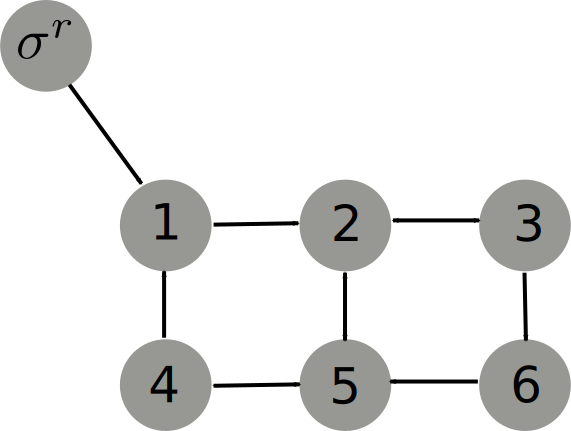
\includegraphics[width=\linewidth]{./images/rat_graph}
\caption{Directed graph.}
\label{fig:rat:sims:graph}
\end{subfigure}
\begin{subfigure}{0.3\linewidth}
\includegraphics[width=\linewidth]{./images/rat_D1_1_3_5_dyn}
\caption{Dynamics.}
\label{fig:rat:sims:dyn}
\end{subfigure}
\caption{Reference attitude tracking.}
\label{fig:rat:sims}
\end{figure}

\begin{figure}
\centering
\begin{subfigure}{0.4\linewidth}
\includegraphics[width=\linewidth]{./images/rat_par_mean}
\caption{Mean - error.}
\label{fig:rat:sims1:mean}
\end{subfigure}
\begin{subfigure}{0.4\linewidth}
\includegraphics[width=\linewidth]{./images/rat_par_var}
\caption{Variance - error.}
\label{fig:rat:sims1:var}
\end{subfigure}
\caption{Comparison on different control parameters.}
\label{fig:rat:sims1}
\end{figure}
